\label{ch::software}
%%%%%%%%%%%%%%%%%%%%%%%%%%%%%%%%%%%%%%%%%%%%%%%%%%%%%%%%%%%%%%%%%%%%%%%%%%%%%%%%%%
%%% Software
%%%
%%% Section 1 : Software Architecture
%%% 
%%% Section 2 : Ground Station
%%%
%%% Section 3 : Simulator
%%%
%%%%%%%%%%%%%%%%%%%%%%%%%%%%%%%%%%%%%%%%%%%%%%%%%%%%%%%%%%%%%%%%%%%%%%%%%%%%%%%%%%
\chapter{Software}
	
	\section{System Software Architecture}
	
	BlueFoot is controlled using a multi-processor software architecture which incorporates several independent core programs. Each of these programs handles portions of system control in a cooperative fashion. Moreover, each of these processors handles specific subsets of operations essential to the macro-system. This distribution of system tasks across several core operating units allows for low-level tasks, such as actuator command and feedback handling, battery monitoring, etc., to be decoupled from more computationally heavy tasks, such as high-level planning and navigation. With task-decoupling in mind, BlueFoot's software architecture was designed such that core programs could be readily offloaded to physically separate computing modules. Each of these control modules handles their own set of assigned tasks in independent control loops. Information is forwarded from each independent processor to update the overall BlueFoot software macro-system in an asynchronous fashion. System control tasks essential to BlueFoot's overall operation are divided into four main categories, which can be summarized as follows:
		\begin{itemize}
			\item{
			\emph{Low-Level Control} : 
				power monitoring / switching, 
				actuator command handling, 
				communications routing,
				sensor data acquisition,
				script parsing and evaluation
			}
			\item{
			\emph{Locomotion Control} : 
				gait planning, 
				gait adaptation, 
				trunk pose adaptation
			}
			\item{
			\emph{High-Level Control} : 
				perception, 
				motion planning, 
				surface reconstruction, 
				navigation, 
				localization
			}
			\item{
			\emph{Human-Operator Control} : 
				joystick/keyboard commands,
				scripting commands
			}
		\end{itemize}
	Low-level and locomotion control tasks are handled, exclusively, by the \emph{Lower Brain} (LB), which designates the software collective spanning over the RM48 and TM4C processors on-board the AutoPilot. High-level control tasks are handled by the Upper Brain (UB), which is a collection of software which runs on the ODROID-XU (ODROID) module. Lastly, a human operator can interface with the system wirelessly from a personal computer running ground-station software. The ground station  communicates with the system through communication lines which enter the TM4C processor and the ODROID computer. The ground-station also interfaces with the UB over an SSH connection. This secondary wireless connection is used, mainly, for on-board data-logging configurations.

	Since this software architecture is distributed over several separate computational units, an integral part of this control architecture is an efficient, reconfigurable interprocessor communication protocol. Namely, BlueFoot utilizes data packets transfered over serial lines to update system states between processors. These data packets are formatted using an in-house designed, binary-XML protocol, called EXI. This protocol facilitates a highly customizable packeting structure for asynchronous inter-module communication and utilizes robust packet-error checking routines. This sections will detail the specifics of BlueFoot's interprocessor communication protocol, namely the composition of packets transferred between processor. 

	This section will also detail the specific software-level tasks handled by each of BlueFoot's processor; the speed at which each core software element is run (update frequency); and what data must be communicated between software elements for operation. Additionally, this section will describe the ground-station software and corresponding user-interface used to control the BlueFoot Quadruped and administer high-level commands.
	
	\subsection{System Task Allocation}

		\begin{figure}[h!]
			\centering
			\fbox{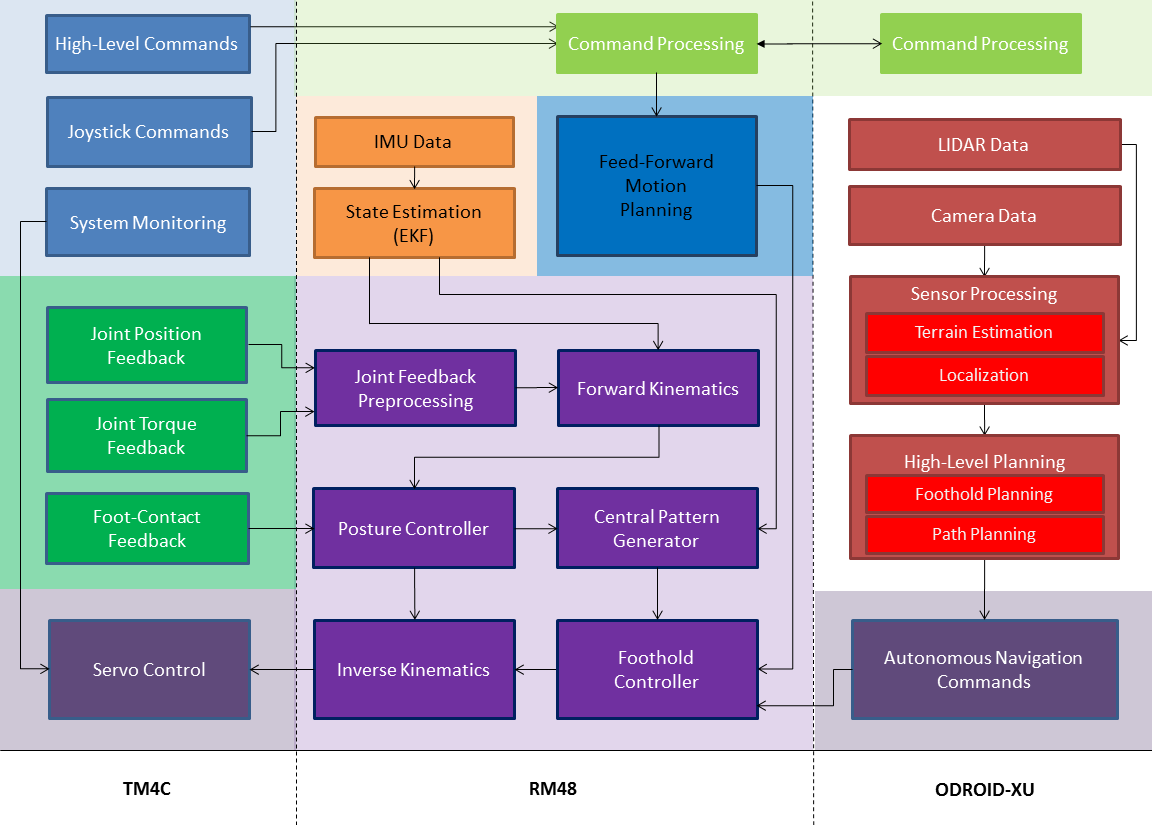
\includegraphics[width=\textwidth]{process_diagram.png}}
			\caption{BlueFoot's on-board processes/signals and their relationships.}
			\label{fig::process_diagram}
		\end{figure}

		Figure \ref{fig::process_diagram} depicts how core software and associated control elements are related within the BlueFoot software macro-system. This section will detail a general description of the tasks carried out by each major software module implemented on the BlueFoot quadruped.

		\subsubsection{TM4C (Lower Brain)}

			As previously mentioned, the TM4C processor on-board the AutoPilot module is responsible for \emph{Low-Level} tasks and can be viewed a safety/communications routing co-processor within the overall system. Within its main program loop, the TM4C polls the system's main battery voltage via ADC interface routines; handles transmit and receive (packet decoding) routines between the ground-station and the RM48 system nodes; and handles command dispatching and feedback polling with the system's 16 servo actuators. The TM4C is directly interfaced with two dual-channel power switching IC's and is used to control power supply to each leg by toggling general purpose IO pins in software. The state of these pins is administered as part of a periodic packet command/update packet sent from the ground-station. Since the TM4C has this control over the system's actuators (which consume most of the system's power) and battery monitoring capabilities, it runs a safety routine which is responsible for halting motor activity and/or cutting system power on low-battery or power-fault conditions, as well as during unexpected breaks in communication with the ground-station.

			As previously mentioned, the TM4C handles communication routing between system processing modules; as well as with controllers on-board each smart-servo. Administering servo commands and collection servo feedback it the TM4C's highest priority task. This process, which involves both commanding and requesting feedback from each servo, is relatively expensive  and limits the TM4C's loop frequency to roughly 50 Hz. Thus, it is particularly important that this task is offloaded to this processor, as its other safety and communication-related tasks are much less expensive, by comparison, and allow the servo actuators to be updated quickly as possible without encumbering other system control operations.


		\subsubsection{RM48 (Lower Brain)}

			The RM48 is responsible for several \emph{Low-Level} tasks, including IMU polling and handling communication with the TM4C and ODROID-XU. Each collected IMU sample is passed along to an extended Kalman Filter routine, which generates a trunk orientation estimate, $\hat{\theta}_{b}$, in the world frame, $O_{0}$. 

			The RM48's primary function is to carry out motion control and gait-planning tasks. To achieve this, the RM48 handles a state machine which switches between planned motion execution and trajectory control; and gait control via a Central Pattern Generator (CPG) based gaiting controller, which will be discussed in more detail in Chapter \ref{ch::gait_control}. Additional functions for body and posture (position and orientation) control, including trunk leveling procedures, and gait-stabilization are run in tandem with the aforementioned gait-control task.

			Motion and gait controls, which are performed in the robot task-space, are converted into joint-space reference angles, $q^{r}$, via an inverse kinematics (IK) routine. The IK routine is executed at all times when the legs are engaged for the purpose of issuing servo position commands, given desired task-space configurations for body and feet positions, which will be more formally defined in Chapter \ref{ch::system_modeling}. The RM48 also maintains BlueFoot's forward kinematic model (specifically, foot position relative to the trunk), which relies on an EKF-generated trunk orientation estimate, $\hat{\theta}_{b}$, and joint position feedback, $q$. BlueFoot's inverse and forward kinematics models will be detailed in Chapter \ref{ch::system_modeling}. The RM48 runs its full control loop at approximatively 100 Hz (twice the speed of the TM4C control loop) to facilitate higher integration stability when updating gait related controller dynamics, dynamic motion controls, task-space reference trajectories.

			Lastly, the RM48 handles an on-board scripting engine (based on the MIT Squirrel scripting language), which interprets lexical commands. This scripting engine is capable of handling a large number of high-level commands and is complex enough to handle function and class definitions in real time \cite{Squirrel_website}. The scripting engine currently being used to evaluate BlueFoot's core user command set, ranging from simple state toggling and parameter modification, to the prescription of user-specified way-points for navigation, among other high-level command items. Scripting commands are passed from the ground station (via terminal) and routed through the TM4C to the RM48, where they are finally evaluated.

		\subsubsection{ODROID-XU (Upper Brain)}

			The ODROID-XU runs software upon a Debian (Linux) operating system distribution ``Jessie." The use of an Linux operating system extends itself to a number of programmatic conveniences, such as to ability to run several tasks in parallel threads. Inbuilt USB drivers are used in functions which are used to acquire data from USB-interfaced vision sensors. Namely, the ORDOID runs sensor handling elements used for acquiring and buffering camera images and controlling camera frame-rate control; as well as LIDAR scan frames. The ORIOID uses these sensor inputs, in conjunction with orientation estimates and inertial data passed from the RM48 to perform several navigation-related tasks (\EG potential fields, mapping, localization, terrain-reconstruction). These tasks will be described in more detail in Chapter \ref{ch::navigation}.

			The ODROID utilizes 2D-LIDAR scans (frames) and trunk-pose estimates to form organized 3D point clouds. These point-clouds are further processed to reconstruct 3D terrain surfaces and height-maps, which are then used for step-planning. LIDAR frames are utilized in potential fields-based navigation tasks. These navigation modes also incorporate camera data for the purpose of goal-targeting (where the goal is typically an object of particular shape or color). Image processing and image feature detection is run as a separate process on the ODROID, which is incorporated with the aforementioned processed sensor data to produce a set of forward and turning velocity commands, $v^{r}$ and $\omega^{r}$, respectively; as well as foot-hold positions generated from step-planning algorithms. In particular, the open-source libraries OpenCV (Open Computer Vision Library), OpenPCL (Open Point-Cloud Library), and Boost are heavily used in the software developed to carry out the aforementioned tasks \cite{opencv_library,openpcl_library,boost_website}. Software written for this platform was generated using a mixture of C++ and Python.

			As previously mentioned, the ODROID can handle a limited set user-command on its own, which are administered directly to the ODROID from an SSH terminal on the ground-station computer. These commands include core-program start-ups and data-logging configurators. Essentially, the ODROID's software core is designed as a completely independent software module which replaces the roll a human director, as it handles the bulk of the systems high-level planning and navigation tasks. Moreover, if the ODROID is removed from the BlueFoot system, the system can still be operated via remote-control heading commands provided from human operator (\IE ground-station joystick control).
		
		\subsection{Inter-processor Communication}

			\begin{figure}[h!]
				\centering
				\fbox{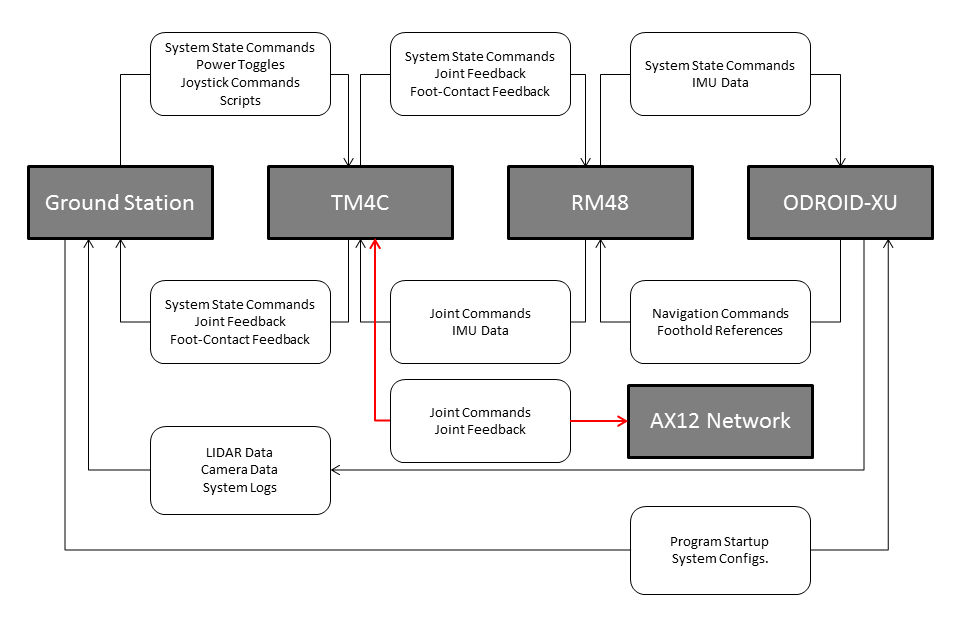
\includegraphics[width=\textwidth]{comm_flow.png}}
				\caption{Communication flow between processors on the BlueFoot Platform.}
				\label{fig::comm_flow}
			\end{figure}

			This section will detail the contents of the data packets transfered between processors, which is summarized in Figure \ref{fig::comm_flow}. System directives, generated by a human operator who interacts with the robot via a graphical user interface and/or joystick controllers, are generated from a ground-station computer. Packets (without padding) sent from the ground station to the BlueFoot robot (TM4C) are composed as shown in Table \ref{tab::gs_to_tm4c_packet}:
			\begin{table}[h!]
				\centering
				\begin{tabularx}{\textwidth}{|C{0.2}|C{0.2}|C{0.2}|C{0.2}|C{0.2}|} 	
					\hline
					\emph{32-bits} 	& \emph{8-bits} 		& \emph{8-bits} 	&\emph{16-bits} 	& \emph{16-bits} 	\\\hline
					HEADER 		& Master-Tog.		& Power-Tog.	& Unused		& Network Info 	\\\hline
					\emph{Variable} 	& 		 		& 			&			& 			\\\hline
					Scripts 		& 				& 			& 			&			\\\hline
				\end{tabularx} 
				\caption{Structure of the packets sent from Ground-Station to TM4C.}
				\label{tab::gs_to_tm4c_packet}
			\end{table}
			
			Every packet issued using the EXI protocol has a 4-byte (32-bit) header. As part of the internal system protocol, every packet sent between system nodes contains a ``Master Status Vector", which is comprised of a fixed length, 7-byte sequence of essential system information and control items. The ``Master Toggles" section (first 8-bits after header) enumerates major systems states, including \emph{On-line, Standby, Off-line} and \emph{Suspended} system state designations. The next 8-bits are used to toggle on-board power, namely the power supplied to each leg. The remaining 32-bits are used for specifying battery voltage (8-bits), power-fault states (8-bits), generic binary feedback toggles (8-bits), and system networking information (16-bits). The last section of this packet contains scripting commands, which can be of varying lengths. For example, forward velocity and turning rate commands (gathered form a joy-stick controller) are administered in the form of scripted commands.

			Packets sent from the TM4C to the Ground-station contain status items generated on board the robot, and appear as shown in Table \ref{tab::tm4c_to_gs_packet}:
			\begin{table}[h!]
				\centering
				\begin{tabularx}{\textwidth}{|C{0.2}|C{0.2}|C{0.2}|C{0.2}|C{0.2}|} 	
					\hline
					\emph{32-bits} 	& \emph{8-bits} 		& \emph{8-bits} 	& \emph{8-bits} 	& \emph{16-bits} 	\\\hline
					HEADER 		& Master-Tog.		& Unused		& Foot-Contacts	& Network Info 	\\\hline\hline
					\emph{2048-bits} 	& 				&			&  			& 		 	\\\hline
					Joint Pos. FB		& 				& 			& 			& 			\\\hline
				\end{tabularx} 
				\caption{Structure of the packets sent from the TM4C to the Ground-Station.}
				\label{tab::tm4c_to_gs_packet}
			\end{table}
			The \emph{Joint Pos. FB} (joint position feedback) element is composed of 16 2-byte sequences corresponding to the joint positions of read-back by each actuator. To avoid redundancy, the structure of the packets communicated from the TM4C to the RM48 and vice-versa will not be depicted explicitly. Like all system packets, these packets contain a 7-byte master status vector with only the \emph{Master-Toggle} and \emph{Network Info} fields populated. The TM4C sends the same joint feedback information to the RM48 as it does the Ground Station. For packets sent from the TM4C to the RM48, this field is replaced with corresponding joint-position commands for each of the 16 servo actuators. This field is also 2048 bits in length.

			Packets sent from the RM48 to the ODROID contain additional dynamical-state fields for use in planning on the ODROID. State information is sent in the form a vectors with 32-bit, single precision floating-point elements. This set of information includes trunk a orientation estimation, angular rate, and global position (generated from open-loop command integration), each of which are represented as 3-element vector; and foot-position estimates (four, 3-element vectors.) generated. These packets have a structure which is depicted in Table \ref{tab::rm48_to_odroid}.
%
			\begin{table}[h!]
				\centering
				\begin{tabularx}{\textwidth}{|C{0.2}|C{0.2}|C{0.2}|C{0.2}|C{0.2}|} 	
					\hline
					\emph{32-bits} 	& \emph{8-bits} 		& \emph{8-bits} 	& \emph{8-bits} 	& \emph{16-bits} 	\\\hline
					HEADER 		& Master-Tog.		& Unused		& Foot-Contacts	& Network Info 	\\\hline\hline
					\emph{96-bits} 	& \emph{96-bits}		& \emph{328-bits}	&\emph{328-bits}  	& 		 	\\\hline
					Orientation		& Angular Rate		& Trunk Pos.		& Foot Positions	& 			\\\hline
				\end{tabularx} 
				\caption{Structure of the packets sent from the RM48 to the ODROID.}
				\label{tab::rm48_to_odroid}
			\end{table}
		Packets sent form the ODROID to the RM48 contain command items, such as forward velocity, turning rate and trunk-pose commands, as well as foothold-references and corrected global trunk position estimates. These packets are constructed as shown in Table \ref{tab::odroid_to_rm48} :
%
			\begin{table}[h!]
				\centering
				\begin{tabularx}{\textwidth}{|C{0.2}|C{0.2}|C{0.2}|C{0.2}|C{0.2}|} 	
					\hline
					\emph{32-bits} 	& \emph{8-bits} 		& \emph{8-bits} 	& \emph{8-bits} 	& \emph{16-bits} 	\\\hline
					HEADER 		& Master-Tog.		& Unused		& Unused		& Network Info 	\\\hline\hline
					\emph{32-bits} 	& \emph{32-bits}		& \emph{96-bits}	&\emph{328-bits}  	& \emph{96-bits} 	\\\hline
					Velocity		& Turning Rate		& Trunk Pose		& Footholds.	& Trunk Pos.		\\\hline
				\end{tabularx} 
				\caption{Structure of the packets sent from the ODROID to the RM48.}
				\label{tab::odroid_to_rm48}
			\end{table}

	\section{Ground Station}
		
		%\begin{figure}[h!]
		%	\centering
		%	\fbox{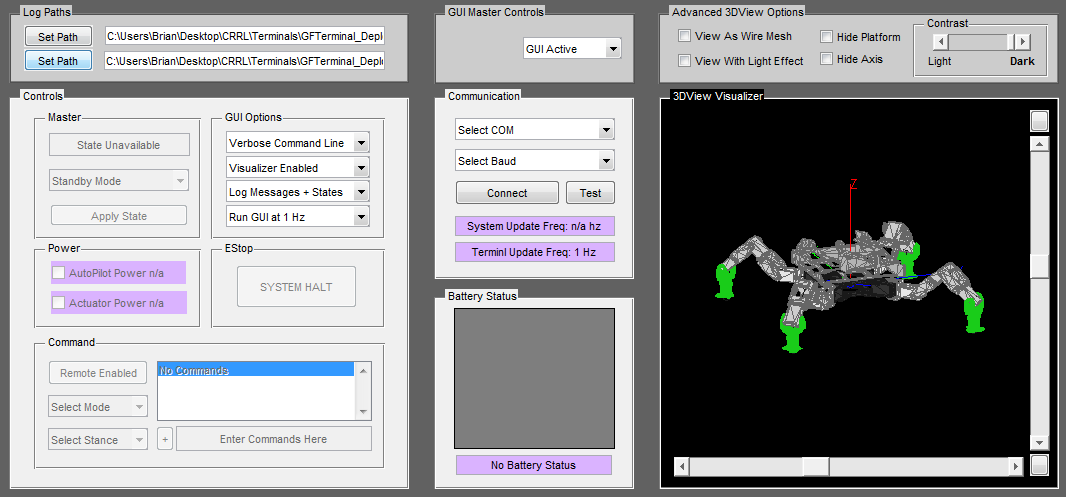
\includegraphics[width=\textwidth]{terminal.png}}
		%	\caption{BlueFoot ground-station GUI}
		%	\label{fig::comm_flow}
		%\end{figure}
		%\begin{figure}[h!]
		%	\centering
		%	%\fbox{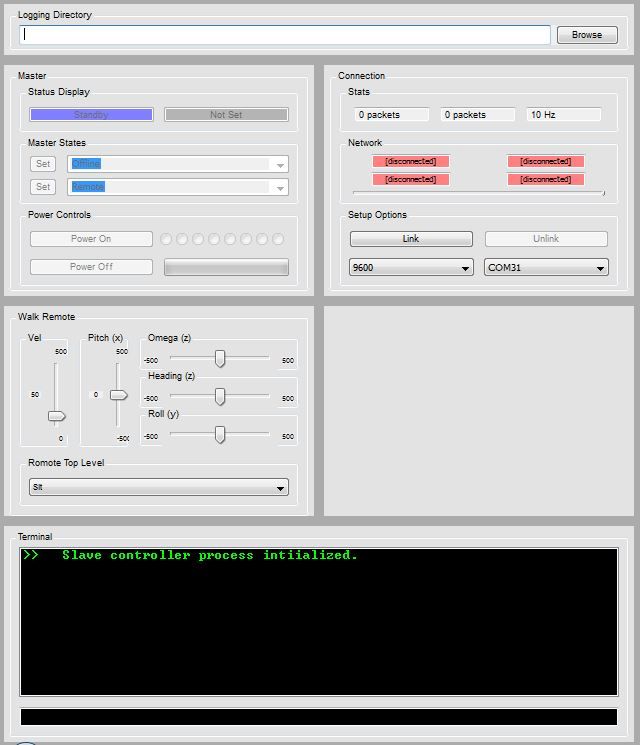
\includegraphics[width=\textwidth]{wxTerminal.jpg}}
		%	\caption{Version 2 of the BlueFoot ground-station GUI, implemented with \emph{wxWidgets}}
		%	\label{fig::comm_flow}
		%\end{figure}s
	Ground-station software used for controlling the BlueFoot platform is generated in C++ using an open-source graphical user interface design library called \emph{wxWidgets} \cite{WX_Website}. \emph{wxWidgets} is used, primarily, for the ground-station's front-end design. Namely, the ground-station code is designed such that that its UI design is reconfigurable via an XML-based design specification file. Furthermore, this allows for UI reconfigurations without the need to change internal, back-end processes. In terms of the GUI back-end, \emph{wxWidgets} handles general UI signal processing, and allows for easy registration of user callbacks on events such as button presses. Additionally, \emph{wxWidgets} provides an interface for collective joystick inputs, which are interpreted and sent to the BlueFoot as remote-control commands. \emph{Boost}, a C++ utility library, is utilized to provide socket and serial-port IO handling. This library is particularly important handling serial-IO ports on the ground station computer, which are used in communicating with the robot over a wireless radio connection.

	The ground station is composed of several main UI sections provide interfaces for administering system master-state, operating-state and power toggling; providing system commands; and scripting. Basic system state controls are used to periodically populate a fixed-structure, robot-command packet, shown in Table \ref{tab::gs_to_tm4c_packet}. This packet is used to refresh the robot operating state and manual navigation commands. Updates from the ground-station are sent to the platform rate of 25 Hz using the an XBEE radio module. BlueFoot replies to each ground-station update with a packet of internal configurations, as shown in Table \ref{tab::tm4c_to_gs_packet}, which is then used to ensure that system updates and commands have been received and that the system is live.

	Namely, BlueFoot sends the following particles of system information back to he ground-station: 
	\begin{itemize}
		\item battery voltage levels 
		\item power fault conditions 
		\item foot contact feedback
		\item and joint position feedback. 
	\end{itemize}
	This data is used to update several key portions of the UI. Firstly, battery levels are used to update a battery meter, which indicates the current system voltage level. Additionally, a dynamic text box displays the system's power-fault state to the user. Joint position commands are used to update a visualization of the robot in real time. The foot-color of the visualized BlueFoot robot changes from blue to red to represent foot-contact conditions. Joint positions, foot-contact states and battery levels are time-stamped and automatically logged during each ground-station session. 

